\documentclass[11pt,a4paper]{article}
\usepackage[margin=2.5cm]{geometry}
\usepackage{graphicx}

\title{Labwork 4: Threads}
\author{Duong Tan Binh \\ Student ID: 2540007}
\date{}

\begin{document}
\maketitle

\section{Method}
I use the same 512 by 600 image and grayscale formula as Lab 3.
The CPU loop and 1D kernel stay the same. In the 2D kernel, I calculate
both x and y from the thread and block indices. Each thread reads
\texttt{src[y, x]} and writes one gray value to \texttt{dst[y, x]}.
I check both coordinates to avoid going outside the image.

I use 2D blocks of 8 by 8, 16 by 16 and 32 by 32 threads.
The grid size is calculated separately for the width and height,
rounding up in each direction.

\section{Results}
I measure each configuration once with \texttt{time.time()}.
Both kernels run once before timing to exclude compilation.
GPU time includes transfers in both directions.
Speedup is CPU time divided by GPU time. I rerun the 1D version with
256 threads per block, using the same image and CPU time for comparison.

\begin{verbatim}
CPU time: 98.982 ms
1D block size: 256
1D time: 0.513 ms
1D speedup: 193.1
2D block size: (8, 8)
2D time: 0.688 ms
2D speedup: 143.8
2D block size: (16, 16)
2D time: 0.43 ms
2D speedup: 230.39
2D block size: (32, 32)
2D time: 0.377 ms
2D speedup: 262.76
\end{verbatim}
The CPU, 1D and 2D versions give the same grayscale values.
Below are the input image, CPU result and 2D GPU result.

\begin{center}
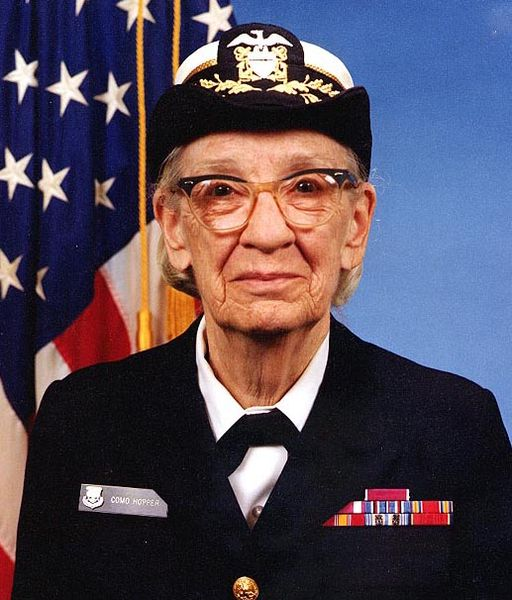
\includegraphics[width=0.23\textwidth]{input.jpg}
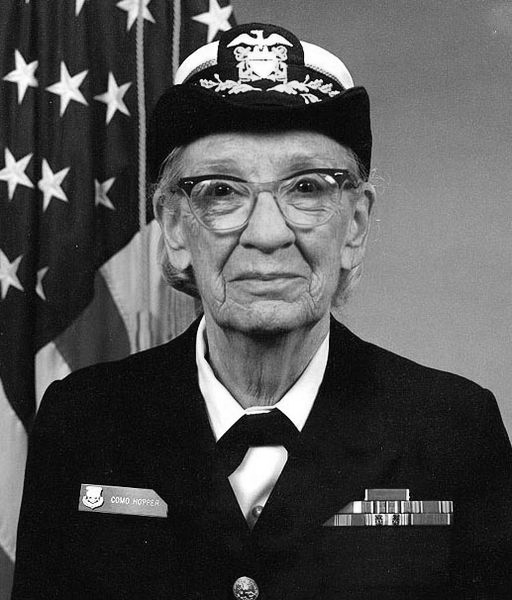
\includegraphics[width=0.23\textwidth]{gray_cpu.png}
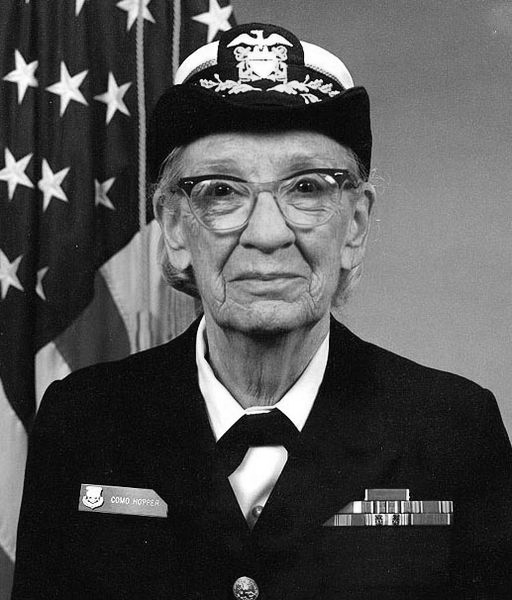
\includegraphics[width=0.23\textwidth]{gray_gpu.png}
\end{center}

\newpage
\section{Comparison}
\begin{center}
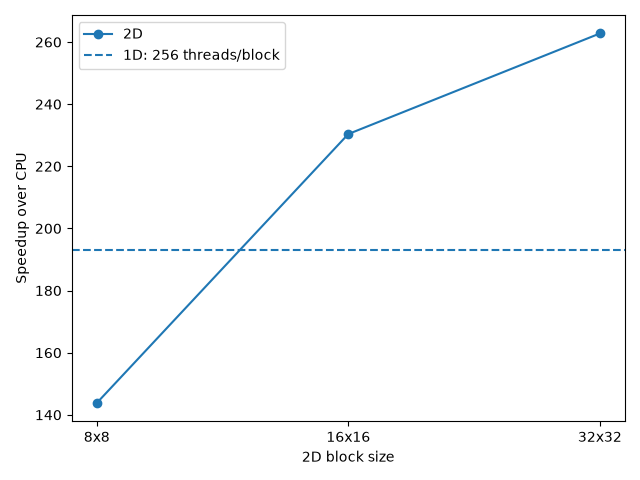
\includegraphics[width=0.75\textwidth]{block_size_speedup.png}
\end{center}
The 32 by 32 block is fastest in this run, with a speedup of 262.76,
compared with 193.10 for the 1D version. The 8 by 8 block is slower
than 1D, so using 2D blocks does not always make this code faster.
These are single measurements and may change between runs.
\end{document}
